\section{Diseño experimental y falsación}

El diseño utilizará pares de semillas comunes cuando sean compatibles, barridos
reducidos, análisis de sensibilidad con intervalo de incertidumbre y preregistro de
criterios de clasificación. El número de réplicas se fijará mediante convergencia y
precisión del estimador, no solo mediante una regla universal de treinta. Para evitar
sesgo por exploración, las configuraciones de confirmación estarán separadas de las
de selección.

\begin{table}[!ht]
\centering
\small
\begin{tabularx}{\textwidth}{@{}c p{4.2cm} X@{}}
\toprule
\textbf{ID} & \textbf{Intervención controlada} & \textbf{Contrafactual y pregunta} \\
\midrule
E0 & Referencia constante, LP fijo, arbitraje activado/desactivado & Verificar existencia
  y naturaleza de un régimen de seguimiento. \\
E1 & Shock exógeno del precio CEX; variar capacidad, costes y retardo & Medir error, cota,
  tiempo de retorno sostenido y resiliencia. \\
E2 & LP estático contra LP adaptativo sensible a volatilidad & Distinguir impacto mecánico
  de menor profundidad de la realimentación endógena. \\
E3 & Presión de ventas y reacciones heterogéneas, mismo shock externo & Identificar
  amplificación, persistencia y límites de la aproximación analítica. \\
\bottomrule
\end{tabularx}
\end{table}

\subsection{Simulaciones preliminares: comprobación de mecanismos}

Se implementó un prototipo sintético reproducible de CPMM, flujo de traders, arbitraje
acotado y LP adaptativo. Se ejecutaron 100 semillas por variante. En E0--E2 se
desactivó el ruido intencionalmente para probar comparativos mecánicos; por ello las
repeticiones coinciden y no deben interpretarse como evidencia estadística
independiente. E3 sí incluye ruido, tendencia y reacción de pánico. No se usaron datos
de mercado: los resultados son una verificación interna de dirección, no validación
externa.

\begin{table}[!ht]
\centering
\scriptsize
\caption{Resultados preliminares sintéticos (medianas de 100 ejecuciones por variante).
Error: $|\log(p^D/p^C)|$.}
\begin{tabularx}{\textwidth}{@{}c >{\raggedright\arraybackslash}p{2.7cm} >{\raggedright\arraybackslash}p{4.5cm} X@{}}
\toprule
\textbf{Escenario} & \textbf{Contrafactual} & \textbf{Resultado observado} &
\textbf{Lectura limitada} \\
\midrule
E0 & Arbitraje activo / apagado & Error máximo 0.0409/0.1000; retorno a banda en
  2/no observado ticks & La corrección acotada reduce el error tras un shock. \\
E1 & Capacidad alta / baja & Retorno a banda en 1/9 ticks; error máximo 0.0030/0.1080 &
  La capacidad de arbitraje importa en la velocidad de recuperación. \\
E2 & LP estático / adaptativo & Impacto de venta fija 0.0940/0.2032; liquidez mínima
  10000/4500 & Menor profundidad aumenta el impacto de la misma venta absoluta. \\
E3 & Liquidez estática / adaptativa & Máximo error 0.0660/0.3719; ticks de retorno 3/33 &
  La regla LP adaptativa puede amplificar una cascada bajo estas condiciones. \\
\bottomrule
\end{tabularx}
\end{table}

En una cuadrícula local de excesos iniciales y órdenes pequeñas, la proyección por
mínimos cuadrados de $d_{t+1}\approx k d_t$ produjo $\hat{k}=0.1874$ bajo
$\gamma=0.003$ y capacidad máxima de arbitraje del 3\% de la reserva por tick; esto
equivale a una contracción diagnóstica $\hat{\alpha}=1-\hat{k}=0.8126$. No se reporta
como parámetro calibrado: cambia con la banda, la capacidad, el tamaño de la orden y
las no linealidades del AMM. Su utilidad en esta etapa es mostrar que la ecuación
reducida puede ser medida contra el propio mecanismo y no solo propuesta de forma
abstracta.

Estos resultados respaldan mantener H1a y H1b como hipótesis operativas. H1c
permanece abierta: aún falta diseñar una clasificación ex ante de los regímenes del
ABM, estimar el mapa en una muestra de selección y evaluarlo en configuraciones de
confirmación separadas.

\begin{figure}[!ht]
\centering
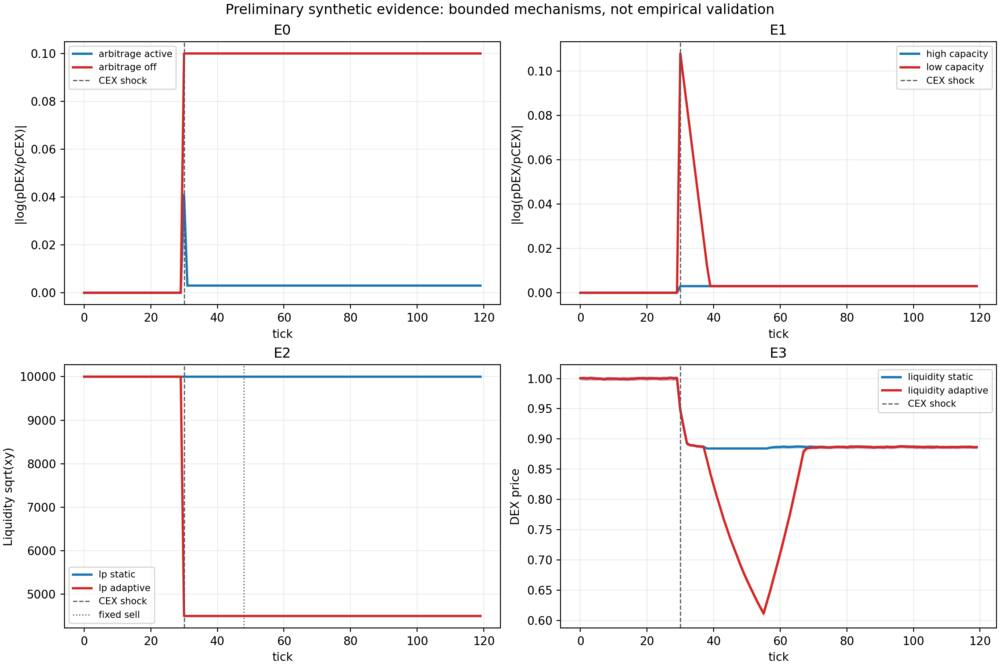
\includegraphics[width=\textwidth]{../figures/preliminary-results.jpg}
\caption{Evidencia sintética preliminar. E0 y E1 muestran el error de seguimiento; E2
muestra el retiro de liquidez antes de una venta fija; E3 muestra la amplificación
transitoria bajo la regla LP adaptativa. Las bandas representan percentiles 25--75
donde existe variación por semilla. El gráfico conserva sus rótulos de origen en inglés:
\emph{arbitrage active/off} significa arbitraje activo/apagado; \emph{high/low capacity},
capacidad alta/baja; \emph{LP static/adaptive}, LP estático/adaptativo; \emph{fixed sell},
venta fija; \emph{liquidity static/adaptive}, liquidez estática/adaptativa; y
\emph{DEX price}, precio del DEX. El título del gráfico indica evidencia sintética de
mecanismos acotados, no validación empírica.}
\end{figure}

\section{Playground reproducible y transferencia tecnológica}

\subsection{Arquitectura}

Un motor determinista de eventos ejecutará el AMM, arbitraje, políticas y contabilidad.
El generador pseudoaleatorio se fijará y sus flujos se separarán por componente; los
shocks y el orden de ejecución serán configurables y registrados. Cada corrida
producirá \texttt{run-id}, archivo de configuración, commit SHA, versión de entorno,
semillas, series temporales, métricas, validación de invariantes y suma criptográfica
de artefactos.

\subsection{Referencia canónica de implementación}

La referencia pública y versionada de la arquitectura es el repositorio
\textit{Master-s-thesis} \cite{calderon2026repository}. En esta versión, el manuscrito
compilable se publica en \texttt{thesis/preprint}; el prototipo CPMM y su análisis se
publican en \texttt{experiments/cex\_dex\_preliminary}. Los destinos de estos enlaces
identifican la arquitectura y sus versiones; los artefactos de cada ejecución conservan
además su propio commit SHA, configuración y semilla. Ninguna rama, URL ni resultado
sintético se interpreta como evidencia empírica de mercado.

\subsection{Contratos de reproducción}

\begin{enumerate}
  \item Configuraciones YAML versionadas, unidades económicas especificadas y
    dependencias bloqueadas (\texttt{uv.lock} o equivalente).
  \item Pruebas de swaps, reservas positivas, inventarios y conservación neta, con
    reglas explícitas para comisiones y retiros.
  \item Comandos estables: \texttt{run one}, \texttt{run sweep}, \texttt{analyze},
    \texttt{verify} y \texttt{reproduce figure}. El prototipo actual se reproduce
    ejecutando \texttt{python3 experiments/cex\_dex\_preliminary/cex\_dex\_preliminary.py}
    con los argumentos \texttt{--output output/preliminary\_simulations --seeds 100}.
  \item CI con simulaciones de referencia y tolerancias numéricas documentadas;
    resultados extensos en almacén de artefactos, no necesariamente en Git.
  \item Dataset sintético como referencia primaria y conjunto empírico acotado con
    licencia, procedencia, timestamps y scripts de ingestión.
\end{enumerate}

\subsection{Relación con software de mercado abierto}

El mercado teórico básico seguirá la mecánica CPMM compatible con un AMM tipo
Uniswap v2 \cite{adams2020uniswap,angeris2020cfmm}; no se extrapolará sin pruebas a
posiciones concentradas de Uniswap v3/v4. Se propone verificar swaps contra contratos
de referencia desplegados localmente con Foundry/Anvil y librerías Web3, bajo
configuración controlada y sin dinero real. Para la referencia CEX se podrán utilizar
series públicas obtenidas con adaptadores de mercado como CCXT o API pública del
exchange, verificando licencias, identidad del par, latencia, spreads y timestamp. Un
segundo nivel, opcional, consiste en replay de eventos on-chain indexados (p. ej.
registros de swaps y Sync de pools compatibles) para validar la magnitud del error de
ejecución. No se requiere correr nodos mainnet, MEV ni trading real.
